\documentclass[11pt,french,a4paper]{article}

\usepackage{graphicx}
\usepackage{listings}
\usepackage{multicol}
\usepackage{titling}
\usepackage{hyphenat}

\usepackage[francais,box,completemulti]{automultiplechoice}
\usepackage{hyperref}
\title{Projet d'intégration de développement}
\date{21/06/2022}
\author{François ROLAND}
\AMCrandomseed{1}
\hypersetup{
  pdftitle={\thetitle},
  pdfauthor={\theauthor},
  pdflang={fr-BE},
  hidelinks}
\usepackage{polyglossia}
\setdefaultlanguage{french}
\usepackage{csquotes}
\geometry{hmargin=2cm,headheight=2cm,headsep=.3cm,footskip=1cm,top=3cm,bottom=2cm}
\begin{document}

%%% preparation of the groups

% chktex-file 19
\setdefaultgroupmode{withoutreplacement}

\element{q001}{
  \begin{questionmult}{objectifs}
    Quels sont les objectifs principaux d'un cahier des charges~?
    \begin{choices}
      \correctchoice{Communiquer le but du projet.}
      \correctchoice{Planifier les moyens à allouer.}
      \correctchoice{Vérifier que le projet est toujours pertinent et que les objectifs sont atteints.}
      \wrongchoice{Dessiner des diagrammes.}
      \wrongchoice{Raccourcir les délais d'analyse.}
      \wrongchoice{S'assurer que le projet ne sera jamais arrêté de manière précoce.}
      \wrongchoice{Éliminer toutes les inconnues du projet.}
    \end{choices}
  \end{questionmult}
}

\element{q002}{
  \begin{question}{diag-contexte}
    Que représente un diagramme UML de contexte~?
    \begin{choices}
      \correctchoice{Les acteurs et la manière dont ils interagissent avec le système.}
      \wrongchoice{Les parties prenantes et la manière dont elles interagissent avec le système.}
      \wrongchoice{Les acteurs et la manière dont ils interagissent dans le projet.}
      \wrongchoice{Les parties prenantes et la manière dont elles interagissent dans le projet.}
    \end{choices}
  \end{question}
}

\element{q003}{
  \begin{question}{acteur-primaire}
    Qu'est-ce qu'un acteur primaire~?
    \begin{choices}
      \correctchoice{Une personne ou un système qui est à l'origine des interactions avec le système.}
      \wrongchoice{Une personne ou un système important.}
      \wrongchoice{Une personne ou un système qui n'est pas directement à l'origine des interactions avec le système.}
      \wrongchoice{Une personne ou un système dont les cas d'utilisation sont traités en priorité.}
    \end{choices}
  \end{question}
}

\element{q003}{
  \begin{question}{acteur-secondaire}
    Qu'est-ce qu'un acteur secondaire~?
    \begin{choices}
      \correctchoice{Une personne ou un système qui n'est pas directement à l'origine des interactions avec le système.}
      \wrongchoice{Une personne ou un système qui est à l'origine des interactions avec le système.}
      \wrongchoice{Une personne ou un système important.}
      \wrongchoice{Une personne ou un système dont les cas d'utilisation sont traités en priorité.}
    \end{choices}
  \end{question}
}

\element{q004}{
  \begin{question}{besoin-fonctionnel}
    \enquote{En tant que bibliothécaire, je veux rechercher un livre sur base du titre et de l'auteur afin de retrouver l'emplacement où il est rangé.}

    De quel type de besoin s'agit-il~?
    \begin{multicols}{3}\AMCBoxedAnswers{}
      \begin{choices}
        \correctchoice{Besoin fonctionnel.}
        \wrongchoice{Besoin non fonctionnel.}
        \wrongchoice{Contrainte.}
        \wrongchoice{Besoin primaire.}
        \wrongchoice{Besoin secondaire.}
      \end{choices}
    \end{multicols}
  \end{question}
}

\element{q005}{
  \begin{question}{singletable}
    Observez le diagramme suivant.

    \begin{center}
      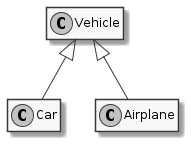
\includegraphics[width=4cm]{class_inheritance.png}
    \end{center}

    En vous basant uniquement sur ces diagrammes, déterminer à quelle(s) classe(s) appartient l'attribut \texttt{altitudeMax}.
    \begin{multicols}{2}\AMCBoxedAnswers{}
      \begin{choices}
        \correctchoice{Les informations fournies ne sont pas suffisantes pour déterminer la classe.}
        \wrongchoice{\texttt{Vehicle}.}
        \wrongchoice{\texttt{Car}.}
        \wrongchoice{\texttt{Airplane}.}
        \wrongchoice{\texttt{Car} et \texttt{Airplane}.}
      \end{choices}
    \end{multicols}
  \end{question}
}


%%% copies

\def\insertRetard{ %
{\AMCquestionNumberfalse%
\def\AMCbeginQuestion##1##2{}\AMCnobloc%
\begin{questionmult}{00retard}
  \AMCnoCompleteMulti\AMCdontAnnotate%
  \def\AMCbeginAnswer{}\def\AMCendAnswer{}%
  Réservé:~\begin{choicescustom}[o]\wrongchoice{retard \(< 5\) minutes~}\scoring{b=0,m=-10}\wrongchoice{retard \(\geq 5\) minutes}\scoring{b=0,m=-20}\end{choicescustom}%
\end{questionmult}}%
}

\onecopy{16}{
  \setlength{\parindent}{0pt}
  %%% beginning of the header
  \begin{minipage}[t]{10cm}
    {\raggedright \LARGE \nohyphens{\thetitle} \par} \vspace{1.5em} {\large \thedate} % chktex 1
  \end{minipage}\hspace{\stretch{1}}%
  \champnom{\fbox{\begin{minipage}[t]{6cm}%
        {\footnotesize Nom et prénom \par}%
        \vspace{8mm}\namefielddots{}%
        \vspace*{1mm}%
      \end{minipage}}}

  \textit{
    \section*{Consignes}
    \begin{itemize}
      \item Répondez aux questions à réponse unique en cochant la case correspondant à la meilleure réponse.
      \item Les questions avec le symbole \multiSymbole{} sont des questions à réponses multiples.
            Cochez toutes les réponses correctes ou cochez la case \enquote{Aucune de ces réponses n'est correcte.}.
      \item Cochez les cases au moyen d'une croix.
      \item En cas d'erreur, noircissez la case sans laisser d'espace blanc.
      \item Rien de ce qui est écrit ou dessiné en dehors des cases à cocher n'est pris en compte pour l'évaluation.
      \item Afin de faciliter la lecture optique, utilisez un bic bleu ou noir.
    \end{itemize}
  }

  \fcolorbox{black}{lightgray}{\insertRetard}
  \vspace*{1cm}

  %%% end of the header

  \cleargroup{all}

  \copygroup[1]{q001}{all}
  \copygroup[1]{q002}{all}
  \copygroup[1]{q003}{all}
  \copygroup[1]{q004}{all}
  \copygroup[1]{q005}{all}

  \insertgroup{all}

  \AMCcleardoublepage{}
}


\end{document}
